\subsection{Comp Ref Voltage Module (CR) }
\label{sec:CR}

The Comp Ref Voltage Module (CR) provides a regulated \SI{1.9}{\volt} supply rail for CO.
As we shall see later, this voltage sets the amount of hysteresis applied to the switching
threshold of the comparator.


\subsubsection{Requirements}

The reference voltage is determined by the computation shown in \ref{threshold}.


\subsubsection{Implementation}


\begin{figure}[h]
    \centering
    \includegraphics[width=0.8\textwidth]{PO/CR/CR}
    \caption{CR - schematic, from datasheet \cite{noauthor_tps783xx_2014}}
\end{figure}

\begin{table}[H]
    \centering
    \begin{threeparttable}[b]
        \begin{tabularx}{\linewidth}{ >
                    {\hsize=.25\hsize}X >
                    {\hsize=0.5\hsize}X >
                    {\hsize=.25\hsize}X  >
                    {\hsize=.5\hsize}X >
                    {\hsize=.25\hsize}X  >
                    {\hsize=3\hsize}X
            }
                  & \multicolumn{4}{c}{pin} &                                                     \\
            \cmidrule(lr){3-6}
            Id    & Net                     & Nb. & Name         & Type           & Function      \\
            \midrule
            $U_1$ & .B                      & 1   & \texttt{IN}  & \leftarrow     & input         \\
            $U_1$ & \Gnd                    & 2   & \texttt{GND} & \Gnd           &               \\
            $U_1$ & EN                      & 3   & \texttt{EN}  & \leftharpoonup & enable output \\
            $U_1$ & \Gnd                    & 4   & \texttt{GND} & \Gnd           &               \\
            $U_1$ & .1V9                    & 5   & \texttt{OUT} & \rightarrow    & output        \\
        \end{tabularx}
    \end{threeparttable}
    \caption{WD - Pin mapping}
\end{table}


\begin{table}[H]
    \centering
    \begin{threeparttable}[b]
        \begin{tabularx}{\linewidth}{
                >{\hsize=0.25\hsize}X
                >{\hsize=0.75\hsize}X
                >{\hsize=1.25\hsize}X
                >{\hsize=0.5\hsize}X
                >{\hsize=2.25\hsize}X}

            Id    & Desc                              & Order Code       & Package       & Rationale \\
            \midrule
            $U_1$ & \cite{noauthor_tps783xx_2014}     & TPS78319DDCR/922 & SOT-23-THIN-5 &           \\
            $C_1$ & \SI{1}{\micro\farad}, \SI{16}{\V} & generic          & 0603          &           \\
            $C_2$ & \SI{1}{\micro\farad}, \SI{16}{\V} & generic          & 0603          &           \\
        \end{tabularx}
    \end{threeparttable}
    % \caption{WD Module - BOM}
    \label{table:wd1}
\end{table}

\begin{table}[H]
    \centering
    \begin{threeparttable}[b]
        \begin{tabularx}{\linewidth}{ >{\hsize=.15\hsize}X >{\hsize=1.35\hsize}X >{\hsize=1.5\hsize}X }

            Id & Issue                                                       & Potential solutions                           \\
            \midrule
            1  & The choice of 1.9V is not ideal, the threshold is too high. & move the comparison function to the \mu C     \\
            1  &                                                             & use a scaling module like SV for more control \\
        \end{tabularx}
    \end{threeparttable}
    \caption{CR - issues}
\end{table}



